\section{Eigenschaften des Lichts}

\subsection{Die Lichtgeschwindigkeit}
\textbf{Lichtgeschwindigkeit im Vakuum}
\[
    c = 299'792'458 \frac{m}{s} \approx 3\cdot10^8 \frac{m}{s}
\]
Alle EM-Wellen breiten sich im Vakuum mit dieser Geschwindigkeit aus \\[2ex]

\textbf{In einem durchsichtigen Medium} (z.B Luft, Wasser, Glas) ist die Lichtgeschwindigkeit geringer als $c$. \\[1ex]
\begin{formulabox}
    \[
        c_n = \frac{c}{n}
    \]
\end{formulabox}
\hspace{5mm} $n = $ Brechungsindex (dimensionslose Materialkonstante)
\\[1ex]

(im sichtbaren Bereich)\\
\begin{tabular}{|c|c|c|c|c|c|}
  \hline
  Medium & Vakuum & Luft & Wasser & Glas & Diamant \\
  \hline
  Brechzahl & 1 & 1.0003 & 1.33 & 1.5 ... 1.7 & 2.4 \\
  \hline
\end{tabular}
\vspace{1mm}

Im Vakuum gilt: $\lambda \cdot \nu = c$ \\[1ex]

Die Frequenz bleibt beim Übergang in ein Medium erhalten (\textbf{Energieerhaltung}) \\[1ex]
\textbf{Wellenlänge im Medium:}
\begin{formulabox}
    \[
        \lambda_n \cdot \nu = c_n \hspace{3mm} \Rightarrow \hspace{3mm} \lambda_n = \frac{\lambda}{n}
    \]
\end{formulabox}

\subsection{Reflexion und Brechung}
\textbf{Reflexionsgesetz:} (gilt für alle Arten von Wellen!)
\begin{formulabox}
    \[
        \Theta_1 = \Theta_1' \hspace{3mm} \text{"Einfallswinkel = Ausfallswinkel"}
    \]
\end{formulabox} 

\textbf{Reflektierte Intensität:} (Spezialfall) $\Theta_1 = \Theta_1' = 0$
\begin{formulabox}
    \[
        I_r = \left( \frac{n_1 - n_2}{n_1 + n_2} \right)^2 I_0
    \]
\end{formulabox}

\textbf{Transmittierte Intensität:}
\begin{formulabox}
    \[
        I_t = I_0 - I_r
    \]
\end{formulabox}

\subsection{Brechungsgesetz}
Beim Übertritt in ein anderes Medium ändert die Lichtwelle ihre Ausbreitungsrichtung, sie wird gebrochen. \\[1ex]
\textbf{Austrittswinkel mit dem Brechungsgesetz:}
\begin{formulabox}
    \[
        n_1 \sin{\Theta_1} = n_2 \sin{\Theta_2} \hspace{3mm} \text{Gesetz von Snellius}
    \]
\end{formulabox}

\textbf{Totalreflexion:}
Ab einem kritischen Einfallswinkel kann beim Auftreffen auf ein Medium ($n_1 > n_2$) eine \textbf{Totalreflexion} auftreten. \\[1ex]

\textbf{kritischer Winkel für Totalreflexion:}
\begin{formulabox}
    \[
        \sin{\Theta_k} = \frac{n_2}{n_1}\sin{90^{\circ}} = \frac{n_2}{n_1}
    \]
\end{formulabox}

\textbf{Dispersion:} \\
Die Brechzahl jedes Mediums hängt (geringfügig) von der Wellenlänge des eintreffenden Lichts ab. In Wellenbereichen, in denen das Material durchsichtig ist, nimmt die Brechzahl typischerweise mit steigender Wellenlänge ab. \\
Effekt $\Rightarrow$ \textbf{Dispersion} \\[1ex]
\begin{center}
    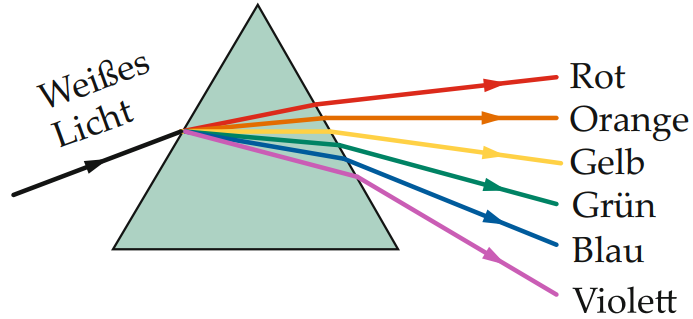
\includegraphics[width=0.50\linewidth]{Abbildungen Physik ZF/Dispersion.png}
\end{center}


\subsection{Polarisation}
EM-Wellen sind Transversalwellen \\[1ex]
- \textbf{lineare Polarisation:} Felder schwingen jeweils entlang einer Achse senkrecht \\ \hspace{5mm} zur Ausbreitungsrichtung \\[1ex]

- \textbf{zirkuläre Polarisation:} Die Spitzen der Feldvektoren beschreiben eine \\ \hspace{5mm} Spirale im Raum \\[2ex]

Mit \textbf{Polaristoren}, die nur eine bestimmte Schwingungsrichtung des $\Vec{E}-$Vektors durchlassen, lassen sich unpolarisierte Wellen linear polarisieren. \\[1ex]

\subsection{Polarisationsmechanismen}
\textbf{1. Absorption:} Richtungsabhängige Absorption in ausgerichteten linearen Molekülen oder Metallfäden, die nicht durchgelassene Polarisationsrichtung wird absorbiert \\ $\rightarrow$ Umwandlung in Wärme \\[1ex]
\textbf{Malusches Gesetz:}
\begin{formulabox}
    \[
        I_2 = I_1 \cos^2{\Theta}
    \]
\end{formulabox}

\textbf{2. Reflexion:} Wenn unpolarisiertes Licht bei einem bestimmten Winkel auf eine ebene Grenzfläche zwischen zwei durchsichtigen Medien triff, stehen der reflektierte und transmittierte Strahl senkrecht aufeinander. $\rightarrow$ reflektierte Welle wird vollständig linear polarisiert
\[
    n_1 \sin{\Theta_p} = n_2 \sin{\Theta_2} = n_2 \sin{(90^{\circ} - \Theta_p)} = n_2 \cos{\Theta_p}
\]
\textbf{Brewster Winkel}
\begin{formulabox}
    \[
        \tan{\Theta_p} = \frac{n_2}{n_1}
    \]
\end{formulabox}

\textbf{3. Streuung:} Reflexion und Absorption von EM-Wellen an Teilchen. Reemittiertes Licht, das in der Ebene senkrecht zur Einfallsrichtung gestreut wird, ist linear polarisiert.

\subsection{Lichtspektrum}
\textbf{Linienspektren:} Valenzelektronen sind für die Energieänderung im Atom zuständig, was zur Absorption führt. Die Energien des aus Atomen emittierten Lichts sind auf bestimmte Wellen beschränkt, was zu den diskreten Spektrallinien führt. \\[1ex]

\textbf{Kontinuierliche Spektren:} Wenn Atome stark miteinander wechselwirken, dann sind viele Energieniveaus der Atome zu ununterbrochenen Bereichen von Energieniveaus verbreitert. Daraus entsteht ein zusammenhängender Bereich \\
$\rightarrow$ kontinuierliches Emissionsspektrum \\[1ex]

\textbf{Sichtbares Licht:} Das menschliche Auge nimmt EM-Strahlung mit Wellenlängen zwischen $\approx 400nm \ - \ 700nm$ wahr. Die entsprechenden Photonenenergien liegen $\approx 1.8 eV \ - \ 3.1eV.$ Sonnenlicht, erscheint als weiss, da es Licht mit allen Wellenlängen in diesem Bereich ist.
